\documentclass{llncs}
\usepackage{todonotes}
\usepackage{url}
\usepackage{hyperref}
\usepackage{graphics}
\usepackage[utf8]{inputenc}
\usepackage[portuguese]{babel}

\begin{document}
\title{Exercício Prático 2: MAPC Agents on Mars}

\author{Alan Rafael Fachini\inst{1} \and Lucas Nascimento\inst{1} \and Márcio F. Stabile Jr.\inst{2}}
\institute{PCS-EPUSP \and IME-USP}

\maketitle

\begin{abstract}
Este relatório descreve a implementação de um time usando a abordagem de sistema multi-agente para a competição no senário ``Agents on Mars'' desenvolvida pelo ``Multi-Agent Programming Contest'' (MAPC) \footnote{\url{http://multiagentcontest.org/2013}}. Neste senários os agentes devem encontrar as melhores zonas com os maiores pesos nos nós do grafo. A implementação apresentada usou como base o sistema ``LTI-USP Team'' desenvolvida por Franco e Sichman \cite{franco2013improving} para a competição de 2013, e testes com estratégias diferentes para a organização dos times foram realizados a fim de tentar identificar estratégias mais eficientes.
\end{abstract}

\section{Introdução}

O “Multi-Agent Programming Contest" (MAPC) é uma competição realizada todos os anos, onde são propostos problemas de domínios variados para a resolução utilizando sistemas Multi-agentes. Seu principal objetivo é o fomento a pesquisa nessa área de estudo. No MAPC, dois times de agentes competem diretamente no mesmo ambiente, oferecendo assim uma oportunidade para a comparação de estratégias e arquiteturas. Desde 2011 o cenário proposto, Agents on Mars, incentiva soluções baseadas em cooperação e coordenação. O objetivo geral do cenário é o controle de zonas em um mapa, representado por um grafo, por se posicionar os agentes em posições, vértices apropriados. A história de fundo do cenário gira em torno da exploração de marte por áreas com concentração de água.

O presente artigo apresenta a estratégia para o time ALM, desenvolvido com base no modelo do time participante da competição de 2013 do Laboratório de Técnicas Inteligentes (LTI) da USP. O time ALM foi desenvolvido como parte da avaliação da disciplina de Sistemas Multi-Agentes pelos alunos Alan Fachini, Lucas Nascimento dos Santos da Silva e Márcio Fernando Stabile Júnior.

\section{System Analysis and Design }

O time ALM foi desenvolvido com base no time LTI-USP participante das competições de 2012 e 2013. O time ALM, assim como o time em que é baseado, utiliza a framework de desenvolvimento para sistemas multi-agentes JaCaMo \cite{jacamo-scp78}. JaCaMo é uma plataforma para a programação de sistemas multi-agentes que suporta vários níveis de abstração (agentes, ambiente, organização). JaCaMo combina três tecnologias para isso: Jason , para programar agentes autônomos; CArtAgO (Common ARTifact infrastructure for AGents Open environments), para programar artefatos do ambiente e Moise, para programar organizações de multi-agentes.

Nenhuma metodologia especifica para o desenvolvimento de sistemas multi-agentes foi utilizada, visto nenhum dos membros possuírem experiência para a mesma e dado o tempo necessário para a conclusão do trabalho.

Baseado no time LTI-USP da versão da competição de 2013, nosso time apresenta uma proposta não centralizada. Apesar de apresentar um agente coordenador, cada agente possui autonomia para decidir quais vértices irá ocupar para criar ou expandir uma zona. Cada agente possui seu modelo interno do ambiente e se comunica com outros agentes para informar a estrutura do mapa, posições dos oponentes ou solicitar reparos. De acordo com as regras da competição de 2013 o time é composto de 28 agentes.

A arquitetura dos agentes é baseada no modelo BDI, com cada agente possuindo sua base de crenças, desejos e intenções. Cada agente tem autonomia para decidir sua próxima ação em cooperação com os demais.

Os agentes se comunicam em forma de broadcast enviando, uns para os outros, mensagens somente em relação às novas percepções recebidas, assim os agentes só enviam mensagens nos casos em que a percepção altera o modelo interno do ambiente do agente. A sobrecarga causada por esse tipo de comunicação no começo da simulação, quando as percepções recebidas pelos agentes são novas, diminui com o progresso da simulação conforme os agentes completam um modelo do ambiente.

O ALM é um sistema multi-agente real no sentido que seus agentes são autônomos, proativos e reativos. São autônomos no sentido de decidir por si próprios qual a próxima ação a ser realizada, ainda que em coordenação com outros agentes e com o agente coordenador. Eles apresentam comportamento proativo quando selecionam o melhor vértice no mapa para se movimentarem. E apresentam comportamento reativo quando, por exemplo, o agente realiza uma recarga ao ficar com baixa energia.

\section{Software Architecture}

A arquitetura do time ALM é a mesma utilizada pelo time LTI-USP na competição de 2013, exibida na Figura \ref{fig:fig1}. Nessa arquitetura foi utilizada a linguagem de programação Jason que provê conceitos de BDI, disponibilizando conceitos abstratos tais como planos, crenças e objetivos. Jason é baseado na plataforma Java e implementa uma extensão da linguagem de programação para agentes AgentSpeak. Jason provê speach acts que são utilizado no trabalho para a comunicação dos agentes. Uma vantagem da utilização da linguagem Jason é a possibilidade de invocar métodos escritos em Java o que permite maior versatilidade na implementação dos agentes e suas ações. Por exemplo, no presente trabalho, conforme descrito anteriormente, a representação interna dos agentes do mundo, ou ambiente, foi implementada em Java na forma de um grafo. Os planos que compõem os agentes são definidos em AgentSpeak, e o agente decide qual plano utilizar de acordo com suas crenças e representação interna do mundo.

O modelo interno do mundo utilizado pelos agentes foi criado em Java usando estruturas de dados e classes, que representam todos os aspectos recebidos do simulador. A cada interação da simulação os agentes atualizam seu modelo interno do mundo de acordo com as percepções recebidas do servidor.


\begin{figure}[!h]
\centering
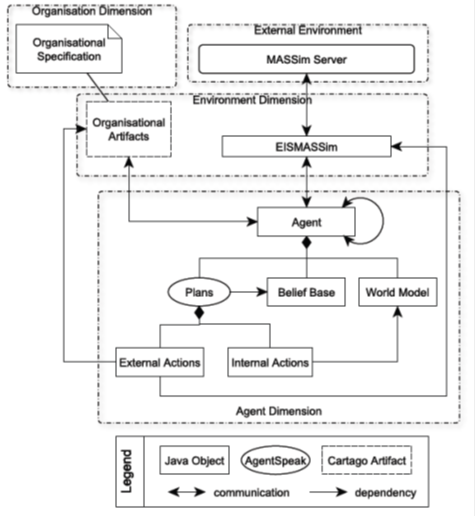
\includegraphics[width=0.7\linewidth]{./Img/fig1.png}
\caption{Arquitetura dos times LTI-USP e ALM.}
\label{fig:fig1}
\end{figure}


A framework CArtAgO foi utilizada para usar os artefatos organizacionais disponíveis em Moise. CArtAgO é uma framework para programação de ambientes baseada em Agentes \& Artifacts (A\&A) para desenhar e modelar sistemas multi-agentes. A framework inclui várias metáforas baseadas em ambientes cooperativos de sociedades humanas, tais como: agentes como entidades computacionais que executam uma tarefa (análogo a trabalhadores humanos); e artefatos, como recursos e ferramentas dinamicamente construídos para o uso e manipulação dos agentes na execução de suas tarefas. Cada artefato pode ser usado e manipulado pelos agentes em tempo de execução. Nesse trabalho não foram desenhados novos artefatos para o uso dos agentes, tal qual o trabalho no qual o presente projeto é baseado os únicos artefatos existentes são os relacionados ao modelo organizacional feito em Moise. 

Moise é um modelo organizacional para sistemas multi-agentes baseado em três dimensões: estrutural, funcional e normativa. 
A dimensão estrutural é construída sob três níveis. O nível individual responde pelo comportamento que um agente adota ao assumir determinado papel. O nível social diz respeito a relação entre papeis e comunicação. E o nível coletivo responde pela agregação de papéis em grupos. 
A dimensão funcional é formada por planos, metas e missões que representam a forma pela qual o sistema multi-agentes alcança o seu objetivo global. O objetivo global é decomposto em planos, que são distribuídos aos agentes na forma de missões, quando um agente recebe uma missão ele se responsabiliza por todas as metas que compõem a missão.
E a dimensão normativa, ou deôntica, abrange a autonomia dos agentes, especificando o que é ou não permitido dentro da organização. A especificação dessa dimensão diz respeito as permissões e obrigações relacionadas a um papel.
O modelo em Moise permite ao desenvolvedor delimitar as restrições da sociedade de agentes, e também pode ser usada para que os agentes raciocinem em relação a sua organização. 
Os agentes se comunicam com o servidor MASSim por meio da interface EISMASSim, baseada em EIS, e distribuída para a competição. Para realizar a comunicação com a interface do servidor para da competição a arquitetura padrão foi alterada para atuar não somente em artefatos do CArtAgO, como também no ambiente EIS.

\section{Strategies, Details and Statistics}\label{sec:strategies}
De acordo com a definição do cenário criada para o MAPC, são definidos cinco tipos diferentes de agentes, cada um com sua especialidade, são: explorador, reparador, sabotador, sentinela e inspetor. Cada classe de agente tem assim um conjunto de ações que lhe são permitidas realizarem, a tabela \ref{table:tab1} exibe qual o conjunto de ações para cada tipo de agente. 

\begin{table}[h]
\centering
\begin{tabular}{|c|c|c|c|c|c|}
	\hline
	         & explorador & reparador & sabotador & sentinela & inspetor \\ \hline
	recharge &      X      &     X      &     X      &    X       & X \\ \hline
	 attack  &            &           &     X      &           &  \\ \hline
	 parry   &            &     X      &    X       &    X       &  \\ \hline
	  goto   &     X       &     X      &   X        &    X       & X  \\ \hline
	 probe   &     X       &           &           &           &  \\ \hline
	 survey  &      X      &     X      &    X       &    X       & X \\ \hline
	inspect  &            &           &           &           &  X\\ \hline
	  buy    &     X       &     X      &     X      &   X        & X \\ \hline
	 repair  &            &      X     &           &           &  \\ \hline
	  skip   &    X        &     X      &    X       &   X        & X \\ \hline
\end{tabular}
\caption{Conjunto de ações por agente.}
\label{table:tab1}
\end{table}

Usando como base o time LTI-USP, os papeis assumidos por nossos agentes não são diretamente mapeáveis para os times definidos para a competição. Assim tipos adicionais de agentes foram definidos de acordo com a estratégia usada. Cada papel tem uma missão associada que pode ser assumida por um ou mais tipos de agente. Segue a descrição dos tipos originalmente definidos para o time LTI-USP:
\begin{itemize}
  \item map\_explorer(explorador): Explora todo o mapa realizando a ação probe em todos os vértices e realizando a identificação de todas as arestas em seu caminho;
  \item map\_explorer\_helper(explorador): Ajuda os agentes do tipo map\_explorer em sua tarefa durante os primeiros 250 passos, posteriormente assume o papel de soldier;
  \item soldier(todos os tipos): Tenta ocupar a melhor área (ou segunda melhor) no ambiente indicada pelo agente coordenador;
  \item guardian(sabotador): Defende a melhor (ou segunda melhor) área de invasores por ataca-los caso se aproximes da área do time ou tentem invadi-la;
  \item medic (reparador): Ocupa o centro da área ocupada e é responsável por reparar os agentes no grupo. Os agentes que precisam de reparos se movem em direção aos agentes medic para serem reparados;
  \item zone\_explorer(explorador): Explora a área ocupada pelo time identificando os vértices cujo valor seja desconhecido. Quando toda área é identifica o zone\_explorer auxilia os agentes soldier a expandir a área ocupada;
  \item saboteur(sabotador): Ataca qualquer agente oponente próximo, ou que esteja ocupando um bom vértice;
  \item sentinel(sentinela): Tenta sabotar o oponente se movendo para dentro da zona inimiga;
  \item repairer(reparador): Segue os agentes do tipo saboteur para realizar reparos, sempre seguindo a duas células de distância para evirar perigo;
  \item coordinator(nenhum): agente interno do sistema que possui um modelo interno do ambiente construído com base nas informações passadas pelos outros agentes. Esse agente determina quais as melhores áreas de ocupação e informa os agentes de sua posição.
\end{itemize}

Em relação ao modelo de agentes utilizado pelo time LTI-USP, o time desenvolvido nesse trabalho muda um pouco a estrutura e os tipos utilizados. Diferente do time LTI-USP nossa abordagem não utiliza os agentes do tipo guardian, optando por uma estratégia mais agressiva. Passamos assim os agentes que estavam sendo usados como guardian para o tipo saboteur com a missão exclusiva de eliminar oponentes. Seguindo essa linha, devido ao maior número de agentes do tipo saboteur atacando preferimos transferir o agente do tipo medic responsável pelo reparo nas zonas ocupadas, para o tipo repairer no grupo de ataque, para prestar assistência aos nossos agentes saboteur. A Figura \ref{fig:fig2} mostra o modelo Moise após essas alterações.

\begin{figure}[!h]
\centering
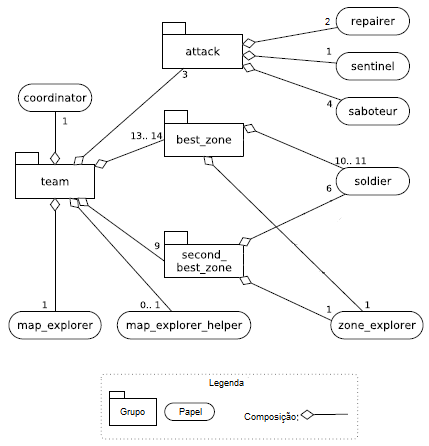
\includegraphics[width=0.7\linewidth]{./Img/fig2.png}
\caption{Modelo Moise dos tipos de agente utilizados pelo time ALM}
\label{fig:fig2}
\end{figure}


\section{Conclusion}
\begin{enumerate}
\item What have you learned from the participation in the contest?
\item Which are the strong and weak points of the team?
\item How suitable was the chosen programming language, methodology,
  tools, and algorithms?
\item What can be improved in the context for next year?
\item Why did your team perform as it did? Why did the other teams perform better/worse than you did.
\item Which other research fields might be interested in the Multi-Agent Programming Contest?
\item How can the current scenario be optimized? How would those optimization pay off?
\end{enumerate}

\newpage
\section*{Short Answers}

Please provide short answers to all the questions in a separate section. This
does not count for the 10 pages limit. Please use the following style for this section:

\begin{verbatim}
\newpage
\section*{Short Answers}
\appendix
\section{Introduction}
\begin{enumerate}
\item What was the motivation to participate in the contest?
\item[A:] Our motiviation was ...
\item What is the (brief) history of the team?
(MAS course project, thesis evaluation, $\ldots$)
\item[A:] In 2006...
\end{enumerate}
\end{verbatim}
Please note: The \verb|A:| stands for "`Answer"'.

\bibliography{references}{}
\bibliographystyle{plain}

\end{document}

